\documentclass{article}

\RequirePackage{units}
\usepackage{amsmath,amsfonts,amssymb,mathtools}
\usepackage[margin=1.2in]{geometry}
\usepackage{graphicx} 
\usepackage{float}
\usepackage{pgfplots}
\usepackage{pgfplotstable}
\usepackage{tikz}
\usetikzlibrary{shapes,arrows,positioning,calc}

\pgfplotsset{width=15cm,compat=1.9}

\title{Kalman Filter for Quadcopter Position Hold}
\author{Peter Davidson and Pantelis Sopasakis}


\begin{document}
\maketitle

\section{Problem statement}
The system dynamics is described by Newton's second law of motion.
Let $z$ be the altitude of the quadcopter, $g$ denotes the acceleration
due to gravity and $a$ is the acceleration that results from the forces
of the propellers. Then, the system dynamics is as simple as
Equation \eqref{eq:newton}
\begin{equation}
    \ddot{z} = a - g.
    \label{eq:newton}
\end{equation}
The acceleration, $a$, is an affine function of the thrust reference signal
(which comes from the RC); it is
\begin{eqnarray}
    a = \alpha \tau + \beta,
\end{eqnarray}
where $\alpha$ and $\beta$ are coefficients to be estimated; we can obtain
\textit{a priori} estimates offline and update them online using measurements
while flying (using the Kalman filter).


@Peter,
\begin{enumerate}
    \item Copy here the system dynamics from Chandra's report (we don't need Section 2.2.3)
    \item Write down what sensors we use and what their characteristics are (level of noise,
          presence of outliers, whether the sensors are biased, update frequencies)
\end{enumerate}
and we'll take it from there.

\newpage
\section{Altitude Dynamics}
The altitude dynamics of a quadcopter are defined within a global coordinate system, crucial for maintaining a predetermined altitude from the Earth's surface. The model that describes these dynamics is based on fundamental principles, delineated as follows:

The rate of change of the quadcopter's altitude, represented as \( \dot{z}_t \), is the result of the vertical acceleration \( a^z_{T_t} \) produced by the drone's motors at a given time minus the gravitational acceleration, \( g \). This equation is continuous in time and is expressed as,
\begin{equation}
\dot{z}_t = a^z_{T,t} - g
\end{equation}
\noindent
Here, \( a^z_{T_t} \) signifies the upward acceleration generated by the propulsion at time \( t \), measured in meters per second squared. The constant \( g \) denotes the acceleration due to Earth's gravity, also in meters per second squared. The altitude \( z_t \) represents the drone's center of mass's vertical position at time \( t \), measured in meters.

Additionally, the drone's vertical velocity \( v_{z_t} \) and vertical acceleration \( a_{z_t} \) are defined by the rate of altitude change \( \dot{z}_t \) and the rate of vertical acceleration change \( \dot{a}^z_{T_t} - g \), respectively. The term \( \dot{a}^z_{T_t} \) is derived from the quadcopter's upward thrust and serves as the system's input, while \( g \) is considered a constant input in the opposite direction.

Let \( y_{t}^z = z_t \) be the output equation of the system. 
Then the corresponding state-space representation is,
\begin{equation}
    \begin{bmatrix}
    v_{v,t}\\
    a_{t}^z
    \end{bmatrix} =
    \begin{bmatrix}
    0 & 1 \\
    0 & 0 
    \end{bmatrix}
    \begin{bmatrix}
    z\\
    v_{v,t}
    \end{bmatrix} + 
    \begin{bmatrix}
    0 & 0 \\
    1 & 1 \\ 
    \end{bmatrix}
    \begin{bmatrix}
    a_{T,t}^z \\ 
    -g
    \end{bmatrix},
    \label{eq:4}
\end{equation}

\noindent
for the barometer sensor's output, denoted by \( y_{barom} \), is described by the equation,
\begin{equation}
y_{barom} = z + d^{bar} + v^{barom}
\end{equation}
where, 
\begin{equation}
    d^{bar}_{t+1} = d^{bar}_t + w_{t}^{d^{bar}}
\end{equation}
The bias $(d^{bar})$ should stay consistent throughout readings, 
the second reading of the bias should be equal to the first allowing for some additional noise/offest.

\noindent
for the GPS sensor's output, 
denoted by \( y^{gps} \), is described by the equation,
\begin{subequations}
    \begin{align}
        y^{\rm gps} 
        {}={}&
        z + v^{\rm gps} 
        \\
        {}={}&
        \begin{bmatrix}
            1 & 0
        \end{bmatrix}
        x + v^{\rm gps} 
    \end{align}
\end{subequations}

The Time-of-Flight (ToF) sensor's output, denoted by \( y^{ToF} \), is described by the equation,
\begin{equation}
y^{\rm ToF} = z + d^{\rm ToF} + v^{\rm ToF}
\end{equation}


Throught all sensors \( y \) represents the output from the sensor. The variable \( z \) signifies the quadcopter's altitude, which is the measurement for all sensors. The term \( v \) encapsulates the measurement noise or errors associated with the sensors. This noise term, \( v \), encompasses various factors such as sensor inaccuracies, the impact of environmental conditions on sensor performance, and any systematic bias that might be inherent in the sensor's readings.

Equation \eqref{eq:4} describes the continuous-time altitude dynamics of the quadcopter. 
The discretization of the altitude dynamics of the system \eqref{eq:4} with a sampling frequency of Ts using the zero-order hold technique is,

\begin{equation}
    \begin{bmatrix}
    z_{t+1}\\
    v_{z,t+1}
    \end{bmatrix} =
    \begin{bmatrix}
    1 & T_s \\
    0 & 1 
    \end{bmatrix}
    \begin{bmatrix}
    z_t\\
    v_{s,t}
    \end{bmatrix} + 
    \begin{bmatrix}
    {1/2}{T^2}_s & {1/2}{T^2}_s \\
    T_s & T_s \\ 
    \end{bmatrix}
    \begin{bmatrix}
    a_{T,t}^z \\ 
    -g
    \end{bmatrix},
\end{equation}




  \section{Modeling}
  The two main forces acting on the quadcopter are the weight, $mg$,
  and the force from the propellers, $F_{\rm prop}$, which has been
  found to depend linearly on the throttle reference signal $\tau\in[0,1]$.
  The throttle reference signal is a signal that is sent to the
  electronic speed controllers (ESCs) of the four motors; at $\tau=0$
  the motors do not spin, whereas $\tau=1$ corresponds to the maximum
  rotation speed.
  
  In an experiment, the quadcopter was placed on digital scales and the
  lift (in $\unit{g}$) was measured for different values of $\tau$.
  The experimental results are shown in Figure \ref{fig:liftpwm}, from
  which it seems that a reasonable model for the lifting force is
  \begin{equation}
    F_{\rm prop} = \alpha \tau + \beta_0,
    \label{eq:Fprop}
  \end{equation}
  where $\alpha_0>0$ and $\beta_0<0$ are constants, which depend on the level of
  charge of the battery. Although the values of $\alpha_0$ and $\beta_0$ can be
  estimated from the data shown in Figure \ref{fig:liftpwm}, their exact
  value is unknown while flying.
  
  From the model of Equation \eqref{eq:Fprop}, the total acceleration is
  \begin{equation}
    a
    {}={}
    \frac{F_{\rm prop} - mg}{m}
    {}={}
    \frac{\alpha_0 \tau + \beta_0 - mg}{m}
    {}={}
    \frac{\alpha_0}{m} + \frac{\beta_0 - mg}{m}
    {}={}
    \alpha \tau + \beta,
  \end{equation}
  where $\alpha = \alpha_0/m$ and $\beta = (\beta_0 - mg) / m$.
  
  As a result, a dynamical model of the system is
  \begin{equation}
    \ddot{z} {}={} a \Leftrightarrow \ddot{z} {}={} \alpha \tau + \beta,
  \end{equation}
  where $z$ denotes the altitude of the quadcopter.
  Note again, that the exact values of the coefficients $\beta$ and $\alpha$ are not known
  while flying (but we will estimate them). We can write this model as
  \begin{subequations}
    \begin{align}
      \dot{z} {}={} & v,
      \\
      \dot{v} {}={} & \alpha \tau + \beta,
    \end{align}
  \end{subequations}
  where $v$ is the quadcopter's vertical velocity.
  By discretising, using Euler's discretisation, with sampling time $T_s$,
  we have
  \begin{subequations}\label{eq:basic-mdl}
    \begin{align}
      z_{t+1} {}={} & z_t + T_s v_t.
      \\
      v_{t+1} {}={} & v_t + T_s(\alpha \tau_t + \beta).
    \end{align}
  \end{subequations}
  The sampling time is $T_s = \unit[100]{ms}$.
  Note that this system is at equilibrium whenever $\alpha \tau_t + \beta = 0$,
  that is, equivalently, $\tau_t = -\beta / \alpha$. This defines the \textit{hovering
    throttle signal}, $\tau^{\rm eq} = -\beta / \alpha$.
  
    \begin{figure}[h]
        \centering
        \begin{tikzpicture}
          \begin{axis}[
              width= 2.2in,
              height=1.2in,
              scale only axis,
              ylabel={Lift (g)},
              xlabel={Throttle reference (\%)},
              xmajorgrids,
              ymajorgrids,
              ylabel near ticks,
              xmin=10, xmax=40,
              ymin=0, ymax=2500,
              legend columns=1,
              legend style={fill=white, fill opacity=0.4, text opacity=1, font=\scriptsize},
              legend style={at={(axis cs:10.5,2450)},anchor=north west},
              legend cell align={left},
            ]
      
            \addplot[mark=x, blue, only marks, line width=1.2pt]
            table
              [x=throttle_percentage, y=weight_decrease, col sep=comma]
              {Data/1045_full.csv};
            \addlegendentry{Full battery ($R^2=99.99\%$)};
      
            \addplot[mark=none, blue!50, only marks, line width=1.2pt, mark=x]
            table
              [x=throttle_percentage, y=weight_decrease, col sep=comma]
              {Data/1045_low.csv};
            \addlegendentry{Low battery ($R^2=90.1\%$)};
      
      
            \addplot[domain=0:50, blue, dashed]
            table
              [x=throttle_percentage, y = {create col/linear regression = {y=weight_decrease}}, col sep=comma]
              {Data/1045_full.csv};
            \addplot[no marks, blue, dashed, domain=0:50]{\pgfplotstableregressiona*x+\pgfplotstableregressionb};
      
            \addplot[domain=0:50, blue!50, dashed]
            table
              [x=throttle_percentage, y = {create col/linear regression = {y=weight_decrease}}, col sep=comma]
              {Data/1045_low.csv};
            \addplot[no marks, blue!50, dashed, domain=0:50]{\pgfplotstableregressiona*x+\pgfplotstableregressionb};
      
          \end{axis}
        \end{tikzpicture}
        \caption{Static lift (g) plotted against throttle reference (\%).}
        \label{fig:liftpwm}
    \end{figure}

    \section{Estimator Design}
    \subsection{State Vector Definition}
    The state vector \( x_t \) is defined as,
    \begin{equation}
        x_t = 
        \begin{bmatrix}
            z_t &
            v_{t} & 
            \beta_t & 
            \alpha_t &
            d{_t}^{\rm bar}&
            d{_t}^{\rm GPS}&
        \end{bmatrix}
    \end{equation}

    \begin{align}
        z_{t+1} =& z_t + {T_s}{v_t} + w^{z}_{t}\\
        v_{t+1}^z =& v_t^z + T_s (\alpha_t \tau_t + \beta_t) + w_t^v\\
        \beta_{t+1} {}={} & \beta_t + w^\beta_t,\\
        \alpha_{t+1} {}={} & \alpha_t + w^\alpha_t.\\
    \end{align}

    We define $w_t^z$ and $w_t^v$ as the process noise elements.
    $w_t^z$ is distributed normally with zero mean and variance
    $\sigma_z^2$, expressed as $w_t^z \sim \mathcal{N}(0, \sigma_z^2)$, 
    and similarly, $w_t^v$ follows a normal distribution with $w_t^v \sim \mathcal{N}(0, \sigma_v^2)$.
    Additionally, $w_t^\alpha$ and $w_t^\beta$ represent white noise processes with distributions
    $w_t^\alpha \sim \mathcal{N}(0, T_s \sigma_\alpha^2)$ and $w_t^\beta \sim \mathcal{N}(0, T_s \sigma_\beta^2)$ 
    respectively. The system's state needing estimation is denoted by $x_t = (z_t, v_t^z, \alpha_t, \beta_t)$, 
    with the The state vector \( x_t \) is defined as,
    \begin{equation}
        x_{t+1} = A_t x_t + w_t^z,
    \end{equation}

    \subsection{State transition matrix \( A_t \)}
    The state transition matrix \( A \) describes how the state at time \( t \) evolves to the state at time \( t+1 \). For the given system.
    Given the state vector \( x_t = \begin{bmatrix} z_t&  v_t^z&  \alpha_t&  \beta_t& d_{bar}& d_{GPS} \end{bmatrix} \), the state transition matrix \( A_t \) from the system's dynamic model is defined as:
    \begin{equation}
    A_t = 
    \begin{bmatrix}
    1 & T_s & 0 & 0 & 0 & 0\\
    0 & 1 & T_s \tau_t & T_s & 0 & 0\\
    0 & 0 & 1 & 0 & 0 & 0 \\
    0 & 0 & 0 & 1 & 0 & 0 \\
    0 & 0 & 0 & 0 & 1 & 0 \\
    0 & 0 & 0 & 0 & 0 & 1 \\
    \end{bmatrix}
    \end{equation}
    where \( T_s \) is the sampling time, and \( \tau_t \) represents the throttle signal at time \( t \).

    \subsection{Process Noise Covariance Matrix \( Q \)}
    The process noise covariance matrix \( Q \) represents the covariance of the process noise, accounting for the uncertainty in the model dynamics:
    \begin{equation}
    Q = 
    \begin{bmatrix}
    \sigma_z^2 & 0 & 0 & 0 & 0 & 0 \\
    0 & \sigma_v^2 & 0 & 0 & 0 & 0 \\
    0 & 0 & T_s \sigma_\alpha^2 & 0 & 0 & 0 \\
    0 & 0 & 0 & T_s \sigma_\beta^2 & 0 & 0 \\
    0 & 0 & 0 & 0 & \sigma^2_{d_{bar}} & 0 \\
    0 & 0 & 0 & 0 & 0 & \sigma^2_{d_{GPS}} \\
    \end{bmatrix}
    \end{equation}
    Here, \( \sigma_z^2 \), \( \sigma_v^2 \), \( \sigma_\alpha^2 \), \( \sigma_\beta^2 \), \( \sigma^2_{d_{bar}} \) and \( \sigma^2_{d_{GPS}} \) represent the variances of the altitude, velocity, and the coefficients \( \alpha \) and \( \beta \), which relate the throttle signal to the lift.

    \subsection{Measurement Matrix \( C \)}
    The measurement matrix \( C \) links the state vector to the measurement vector:
    \begin{equation}
    C = 
    \begin{bmatrix}
    1 & 0 & 0 & 0 & 0 & 0 \\
    1 & 0 & 0 & 0 & 0 & 1 \\
    1 & 0 & 0 & 0 & 1 & 0 \\
    \end{bmatrix}
    \end{equation}
    This matrix considers the direct measurement of altitude by all sensors and accounts for biases in the GPS and barometer sensors.

    The measurement model is defined as
    \begin{equation}
    y_t = C x_t + e_t
    \end{equation}
    \begin{equation}
        y_t  = 
        \begin{bmatrix}
            1 & 0 & 0 & 0 & 0 & 0 \\
            1 & 0 & 0 & 0 & 0 & 1 \\
            1 & 0 & 0 & 0 & 1 & 0 \\
        \end{bmatrix}
            x_t + e_t
    \end{equation}
    \subsection{Measurement Noise Covariance Matrix \( R \)}
    The measurement noise covariance matrix \( R \) accounts for the uncertainty in sensor measurements:
    \begin{equation}
    R = 
    \begin{bmatrix}
    \sigma_{barom}^2 & 0 & 0 \\
    0 & \sigma_{gps}^2 & 0 \\
    0 & 0 & \sigma_{ToF}^2
    \end{bmatrix}
    \end{equation}
    where \( \sigma_{barom}^2 \), \( \sigma_{gps}^2 \), and \( \sigma_{ToF}^2 \) are the variances of the measurement noises for the 
    barometer, GPS, and Time-of-Flight sensors, respectively.


    \section{Kalman filter equations}
The Kalman filter equations for the above system are:
\begin{align}
  \text{Measurement} &
  \left[
  \begin{array}{l}
    \hat{x}_{t{}\mid{}t}
    {}={}
    \hat{x}_{t{}\mid{}t-1}
    {}+{}
    \Sigma_{t{}\mid{}t-1}C^\intercal 
    (C\Sigma_{t{}\mid{}t-1}C^\intercal +R)^{-1}(y_t - C\hat{x}_{t{}\mid{}t-1})
    \\
    \Sigma_{t{}\mid{}t}
    {}={}
    \Sigma_{t{}\mid{}t-1}
    {}-{}
    \Sigma_{t{}\mid{}t-1}C^\intercal 
    (C\Sigma_{t{}\mid{}t-1}C^\intercal + R)^{-1}
    C\Sigma_{t{}\mid{}t-1}
  \end{array}
  \right.
  \\
  \text{Time update}        &
  \left[
  \begin{array}{l}
    \hat{x}_{t+1{}\mid{}t}
    {}={}
    A_t \hat{x}_{t{}\mid{}t}
    \\
    \Sigma_{t+1{}\mid{}t}
    {}={}
    A_t \Sigma_{t{}\mid{}t} A_t^\intercal + Q
  \end{array}
  \right.
  \\
  \text{Initial conditions} &
  \left[
  \begin{array}{l}
    \hat{x}_{0{}\mid{}-1}
    {}={}
    \tilde{x}_0
    \\
    \Sigma_{0{}\mid{}-1}
    {}={}
    P_0
  \end{array}
  \right.
  \end{align}

  \subsection*{Measurement Update (Correction Step):}
  The first equation represents the update of the state estimate $\hat{x}_{t|t}$. It is a corrected estimate based on the new measurement 
  $y_t$. The term $\hat{x}_{t|t-1}$ is the predicted state from the previous timestep, and $C$ is the measurement matrix that relates the state 
  to the measurement. The product $C\Sigma_{t|t-1}C^\intercal + R$ is the predicted measurement covariance, and $R$ is the measurement noise 
  covariance matrix. The entire term $(C\Sigma_{t|t-1}C^\intercal + R)^{-1}(y_t - C\hat{x}_{t|t-1})$ is the Kalman gain multiplied by the measurement 
  residual (the difference between the actual measurement and the predicted measurement). The second equation updates the estimate covariance $\Sigma_{t|t}$,
   which measures the estimated accuracy of the state estimate. This step essentially adjusts the estimated covariance to account for the new measurement.

  \subsection*{Time Update (Prediction Step):}
  The third equation predicts the state $\hat{x}_{t+1|t}$ at the next timestep, based on the current corrected state estimate $\hat{x}_{t|t}$. The matrix
   $A_t$ is the state transition model which is applied to the current estimate. The fourth equation predicts the state covariance $\Sigma_{t+1|t}$ for the 
   next timestep. This prediction includes the process noise $Q$, which accounts for the uncertainty in the prediction model.

  \subsection*{Initial Conditions:}
  These two equations provide the initial state estimate $\hat{x}_{0|-1}$ and initial estimate covariance $\Sigma_{0|-1}$ before any measurements are made. 
  $\tilde{x}_0$ is the initial state estimate, and $P_0$ is the initial estimate covariance. These conditions are necessary to start the recursive Kalman filter process.

  \section{Simulations}
  Initially we designed and ran simulations with estimations on both \(alpha\) and \(beta\)

  \begin{figure}[h]
    \centering
    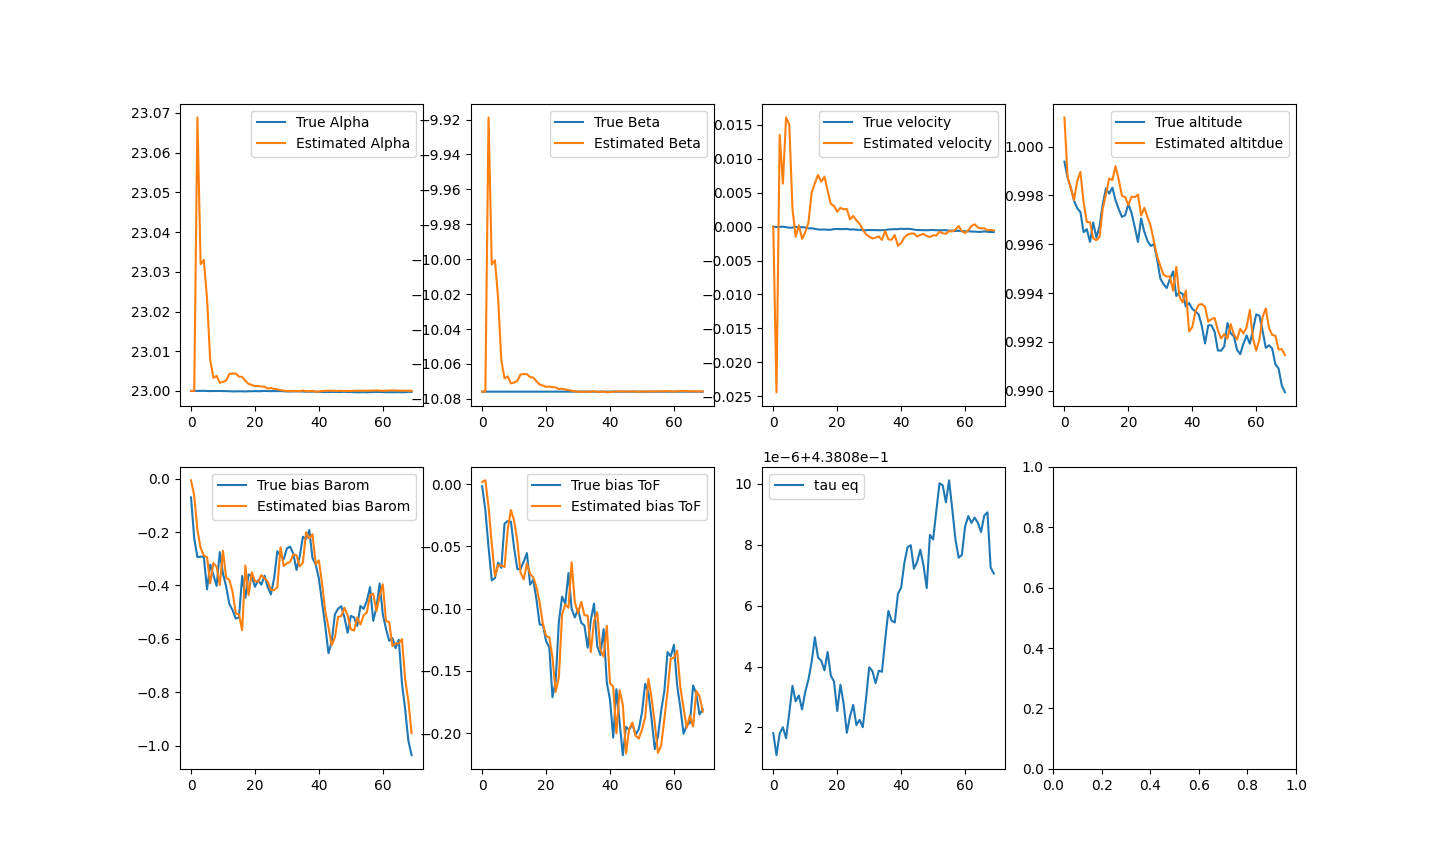
\includegraphics[width=0.7\textwidth]{no_constant.png}
    \caption{Simulations estimating both \(alpha\) and \(beta\)}
    \label{fig:no_constant}
  \end{figure}
  As you can see from the graphed simulation data above we are estimating both \(\alpha\) and \(\beta\) as well as the velocity, altitude and bias for the barometer and tof module.
  All data estimates converge to the true value quickly making for a successful simulation. the values we used for.... are....



  \begin{figure}[h]
    \centering
    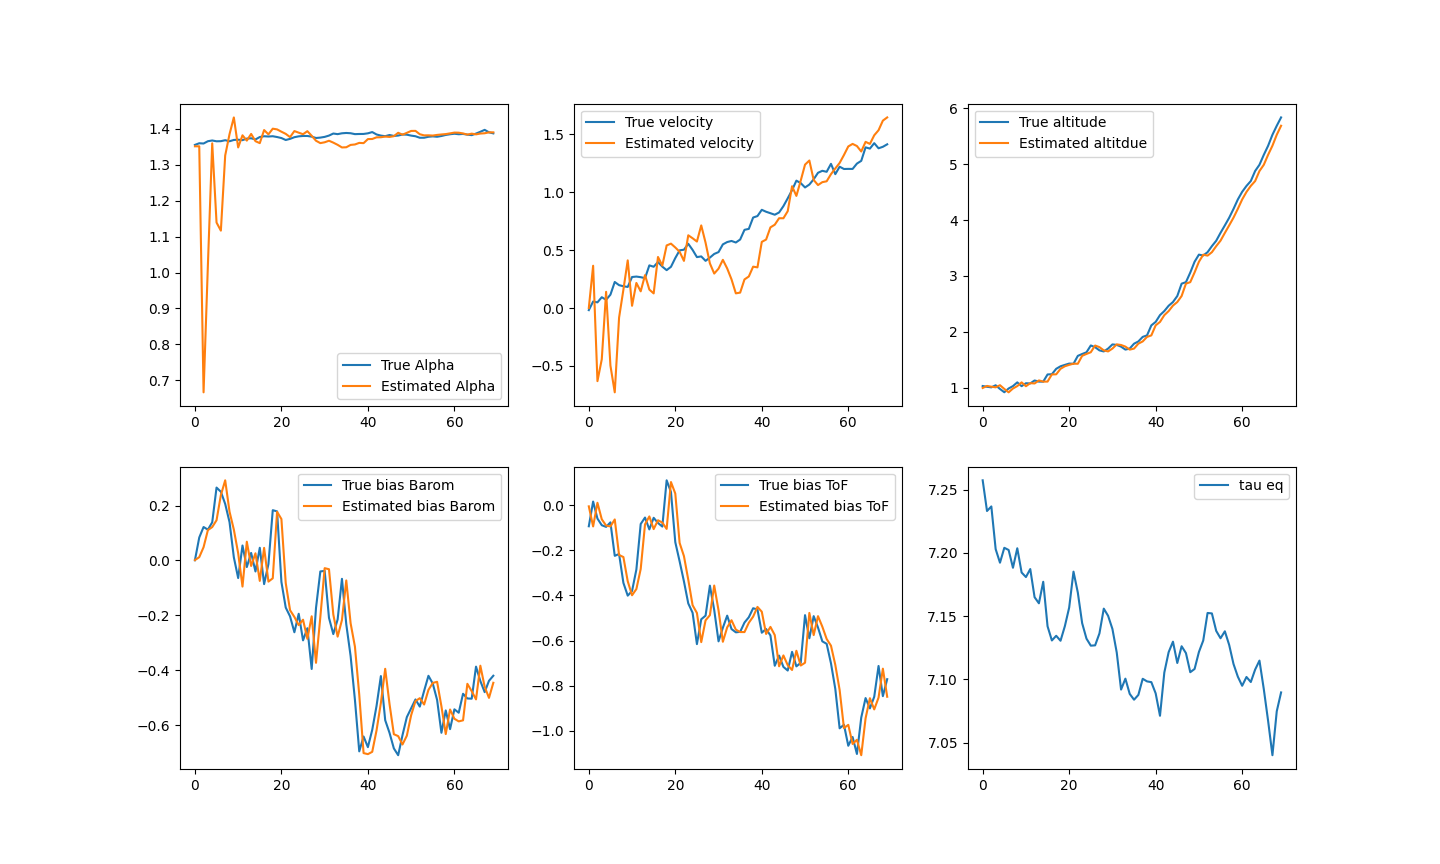
\includegraphics[width=0.7\textwidth]{b_constant.png}
    \caption{Simulations estimating only \(alpha\) whilst \(beta\) is constant}
    \label{fig:b_constant}
  \end{figure}

  \begin{figure}[h]
    \centering
    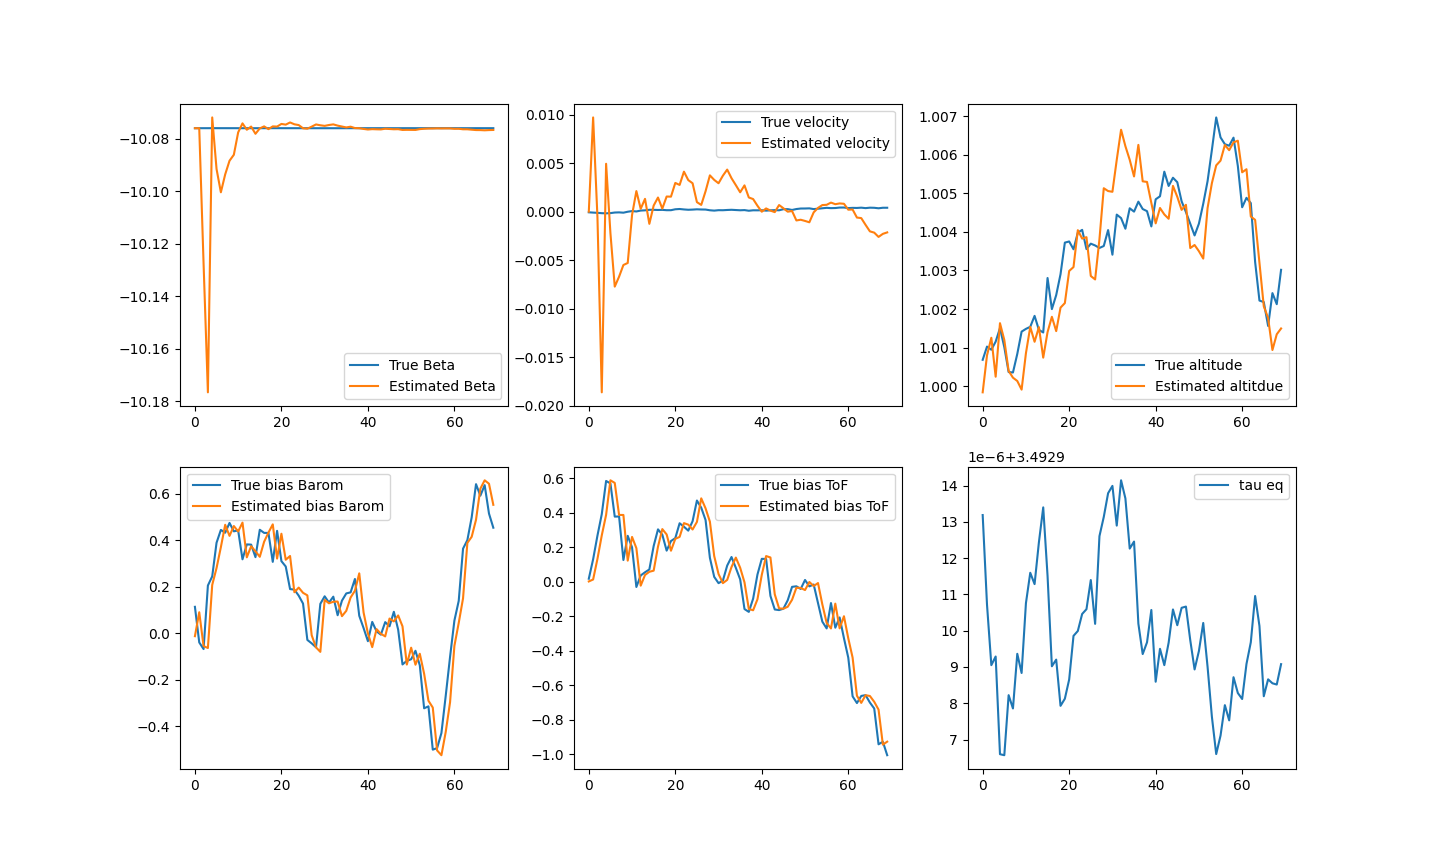
\includegraphics[width=0.7\textwidth]{a_constant.png}
    \caption{Simulations estimating only \(beta\) whilst \(alpha\) is constant}
    \label{fig:a_constant}
  \end{figure}

  \end{document}
        